% Drawing 144/06-1 -- folder 144, batch 06, archive page 102 (PDF page 103).
% Transcription: Une sphère (la droite projective complexe) : un grand cercle horizontal portant les points $0$, $1/2$, $1$, $2$, $-1$, le point $\infty$ marqué sur la face arrière ; un méridien passant par $1/2$ ; un fuseau hachuré entre deux méridiens.
% Kind: Riemann sphere: great circle with 0, 1/2, 1, 2, -1, infinity; meridian; hatched lune. Method 2 (schematic redraw from the facsimile). Status: ok.
% Notes: Re-read on a tight crop; points placed once. The outline (doubled on the page, drawn once). The tilted great circle: its front half solid from 0 through 1/2 to 1, its back half dashed through 2, infinity (big dot) and -1 to the left edge, where it joins the solid hook that closes it at 0. The meridian through 1/2, reinforced, drawn through the point 1/2; the dashed back meridian through 2; the reinforced left meridian from the top through the left edge to 0, dashed below 0 to the bottom. The lune between the left meridian and the meridian through 1/2 carries six near-horizontal hatching strokes, as on the page. Labels \small: 0, 1/2, 1, 2, -1, infinity. The "1b" and the text at the top right are not part of the figure. Redrawn 2026-11-09 (issue 128): to check again. Overlay check 2026-11-13 (issue 147, Claude Opus 5.5): the redraw, rasterised from its TikZ paths, laid over the 300 dpi colour render of the 250 ppi scan with the contrast raised. Redrawn from the page where it was off: the outline is a closed curve through points read on the pencil (the ellipse ran up to 3 units inside it at the upper left and upper right), with the second stroke of the outline at the lower left; the six hatching strokes are drawn where they are, each from its own left end (at 35, 40, 44, 49, 61 and 69 units down; the topmost of the old set was the heavy top of the outline, and the stroke at 35 was missing), the third and fourth stopping short of the meridian through 1/2, the fifth faint and broken on the page; the meridian through 1/2 follows its ink (up to 1.7 units right of the old line below the equator); the back half of the great circle runs through its dashes (lower on the left); the dashed path from 0 to the foot of the meridian runs through its dashes; the left meridian now also goes on, heavy, from the left edge straight down to 0, as on the page, besides the hook. Every stroke lies on its ink to within about 1 unit; the dashed strokes cover their dashes. Kept: the front half of the great circle is gone over twice between 0 and 1/2 and drawn once. Not compiled (no TeX engine in the session).
% Coordinates: 1 unit = 1 mm = 1/100 of the crop width (bbox in page fractions: [0.13, 0.06, 0.47, 0.31]).
% Redrawn by Claude (claude-opus-5-5), issue #73, 2026-11-09; not checked by a human; not compiled (no TeX in the session).
% Checked by Claude (claude-opus-5-5) 2026-11-13 (issue #147): overlay on the 300 dpi colour render of the 250 ppi scan (contrast raised), redrawn in part; not compiled (no TeX in the session). Not checked by a human. Status: ok.
% Rights: reproduces part of the work -- behind RENDER_TRANSCRIPTS, never published by itself.
\documentclass[tikz,border=3pt]{standalone}
\usepackage{amsmath,amssymb}
\usetikzlibrary{patterns,arrows.meta}
\tikzset{pencil/.style={black!45}, struck/.style={black!35}, mark/.style={circle,draw,inner sep=1.3pt}, pt/.style={circle,fill,inner sep=0.9pt}, opt/.style={circle,draw,fill=white,inner sep=1.1pt}}
\begin{document}
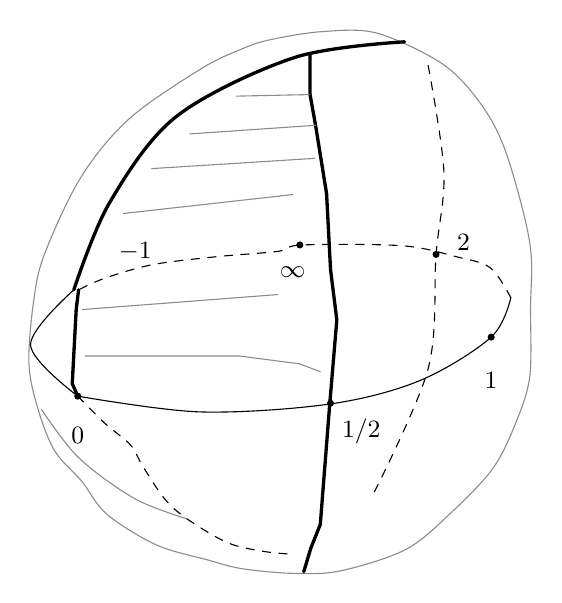
\begin{tikzpicture}[x=1mm,y=1mm,line cap=round,line join=round,font=\scriptsize]
\draw[pencil] plot[smooth cycle, tension=0.55] coordinates {(48.6,-27.2) (55.5,-27.4) (63.8,-31.3) (68.7,-36.4) (71.9,-42.6) (74.9,-54) (75,-62.4) (74.9,-71) (73.2,-76.7) (70.2,-82.7) (64.7,-88.5) (59.1,-93) (50.8,-95.7) (44.7,-96) (38.3,-95.4) (34,-94.3) (27.5,-92.4) (21.2,-88.5) (18,-84.3) (14.6,-80.5) (12.5,-75.3) (11.3,-69.4) (11.9,-61.4) (13.3,-55.4) (17.9,-45.7) (24,-38.3) (33.2,-31.9) (38.6,-29.3) (42.1,-28.2)};
\draw[pencil] plot[smooth, tension=0.55] coordinates {(31.4,-89.1) (24.7,-86.5) (17.6,-81.3) (12.9,-75.2)};
\draw plot[smooth, tension=0.55] coordinates {(17.5,-73.5) (33,-75.5) (49.5,-74.5) (61,-71.5) (70,-66) (72.5,-61)};
\draw[dashed] plot[smooth, tension=0.55] coordinates {(72.5,-61) (69.9,-57.2) (65.6,-55.8) (58.7,-54.4) (46,-54.3) (43,-55.1) (35,-55.8) (27,-56.8) (21,-58.5) (17.6,-60)};
\draw[very thick] (47,-30) -- (47,-35.2) -- (47.7,-39.1) -- (49.1,-47.8) -- (49.6,-57.4) -- (50.4,-63.8) -- (49.5,-74.5) -- (48.3,-89.8) -- (47.1,-92.8) -- (46.2,-95.8);
\draw[dashed] plot[smooth, tension=0.55] coordinates {(62,-31.5) (64,-45) (63,-55.5) (62,-70) (55,-86)};
\draw[very thick] plot[smooth, tension=0.55] coordinates {(59,-28.5) (45,-30.5) (30,-38) (21.5,-49) (17,-60)};
\draw plot[smooth, tension=0.55] coordinates {(17,-60) (11.5,-67) (17.5,-73.5)};
\draw[very thick] (17.6,-60) -- (17.3,-62.5) -- (16.8,-71.9) -- (17.5,-73.5);
\draw[dashed] plot[smooth, tension=0.55] coordinates {(17.5,-73.5) (21,-77) (24.2,-79.7) (25.7,-82.3) (28.5,-86.5) (31.4,-89.1) (36.5,-92.1) (41,-93.2) (45,-93.6)};
\draw[pencil] (37.6,-35.4) -- (46.9,-35.2);
\draw[pencil] (31.7,-40.2) -- (47.7,-39.1);
\draw[pencil] (26.9,-44.6) -- (47.6,-43.3);
\draw[pencil] (23.3,-50.3) -- (44.8,-47.9);
\draw[pencil] (18.1,-62.5) -- (42.9,-60.6);
\draw[pencil] (18.4,-68.4) -- (38,-68.4) -- (45.7,-69.4) -- (48.3,-70.4);
\node[pt] at (17.5,-73.5) {};
\node[pt] at (49.6,-74.4) {};
\node[pt] at (70,-66) {};
\node[pt] at (63,-55.5) {};
\node[pt] at (45.7,-54.3) {};
\node[inner sep=1pt] at (17.5,-78.5) {\small $0$};
\node[inner sep=1pt] at (53.5,-78) {\small $1/2$};
\node[inner sep=1pt] at (70,-71.5) {\small $1$};
\node[inner sep=1pt] at (66.5,-54) {\small $2$};
\node[inner sep=1pt] at (24.8,-55.2) {\small $-1$};
\node[inner sep=1pt] at (44.8,-57.7) {\small $\infty$};
\end{tikzpicture}
\end{document}
